\documentclass[dvipsnames,border=3pt]{standalone}
\usepackage{tikz}
\usetikzlibrary{arrows}
\usetikzlibrary{shapes}
\usepackage{enumitem}
\usepackage{bm}
\usepackage{mathdots}
\usepackage{amsmath}
\usetikzlibrary{shadings}
\usetikzlibrary{decorations.pathreplacing}
\usepackage{helvet}
\usetikzlibrary{arrows.meta}
\usepackage{graphicx}
\usepackage{pgfplots}
\usepackage{pgfplotstable}
\usepackage{filecontents}
\usetikzlibrary{plotmarks}
\pgfplotsset{compat=newest}

\renewcommand{\familydefault}{\sfdefault}

\definecolor{mylightgray}{cmyk}{0,0,0,0.1}
\usetikzlibrary{arrows,decorations.pathmorphing,backgrounds,fit,positioning,shapes.symbols,chains}

\begin{document}

\begin{tikzpicture}
    % trim=left botm right top
    
    \node at (4.5,2.4) {\LARGE \textbf{Correlated data with main effects}};
    
    \draw[-latex, line width=1mm,draw=gray!70] (3.62,0) -- (5.23,0);
    
    \draw[-latex, line width=1mm,draw=gray!70] (9,-1.76) -- (9,-3.4);
    
    \draw[-latex, line width=1mm,draw=gray!70] (5.79,-5.85) -- (2.62,-5.85);
    
    \draw[-latex, line width=1mm,draw=gray!70] (1.5,-6.53) -- (1.5,-9.83);
    
    \node at (0,0) {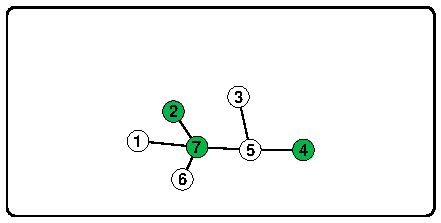
\includegraphics[clip,trim=0.1cm 0.1cm 0.1cm 0.1cm]{interaction_simulation1.pdf}};
    
    \node at (9,0) {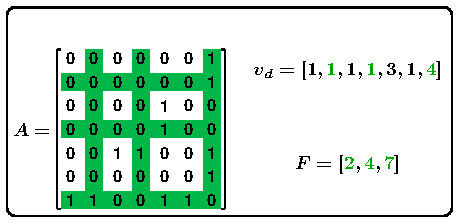
\includegraphics[clip,trim=0.1cm 0.1cm 0.1cm 0.1cm]{interaction_simulation2.pdf}};
    
    \node at (9,-5.85) {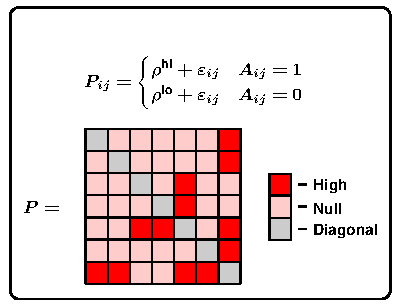
\includegraphics[clip,trim=0.1cm 0.1cm 0.1cm 0.1cm]{main_plus_correlation3.pdf}};
    
    \node at (0,-5.85) {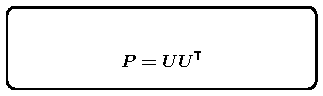
\includegraphics[clip,trim=0.1cm 0.1cm 0.1cm 0.1cm]{main_plus_correlation4.pdf}};
    
    \node at (4.5,-12.92) {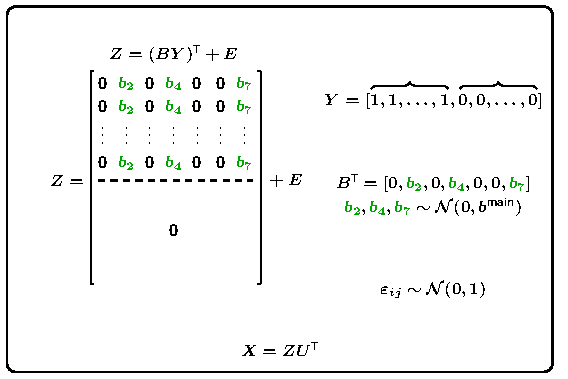
\includegraphics[clip,trim=0.1cm 0.1cm 0.1cm 0.1cm]{main_plus_correlation5.pdf}};
    
    %%%%%%%%%%%%%%%%%%%%%%%%%%%%%%%%%%%%%%% box 1 %%%%%%%%%%%%%%%%%%%%%%%%%%%%%%%%%%%%%%%%%%%%%%%
    \node[circle,draw,line width=0.2mm,xscale=1.4,yscale=1.4,fill=gray!40] at (-3.3,1.45) {};
    \node at (-3.3,1.45) {\textbf{1}};
    
    \node[xscale=1,yscale=1] at (0,0.9) {\textbf{Erd\H{o}s-R\'{e}nyi or Scale-free}};
    %\node[xscale=1,yscale=1] at (2.28,0.9) {\textbf{Erdos-Renyi}};
    %\node[xscale=1,yscale=1] at (0,0.9) {\textbf{or}};
    \node[xscale=1,yscale=1] at (0,1.45) {\textbf{Random graph}};
    %%%%%%%%%%%%%%%%%%%%%%%%%%%%%%%%%%%%%%% box 1 %%%%%%%%%%%%%%%%%%%%%%%%%%%%%%%%%%%%%%%%%%%%%%%
    
    %%%%%%%%%%%%%%%%%%%%%%%%%%%%%%%%%%%%%%% box 2 %%%%%%%%%%%%%%%%%%%%%%%%%%%%%%%%%%%%%%%%%%%%%%%
    \node[circle,draw,line width=0.2mm,xscale=1.4,yscale=1.4,fill=gray!40] at (5.55,1.45) {};
    \node at (5.55,1.45) {\textbf{2}};
    
    \node[xscale=1,yscale=1] at (7.5,1.45) {\textbf{Adjacency matrix}};
    \node[xscale=1,yscale=1] at (11,1.2) {\textbf{Degree vector}};
    \node[xscale=1,yscale=1] at (11,-0.4) {\textbf{Functional features}};
    %%%%%%%%%%%%%%%%%%%%%%%%%%%%%%%%%%%%%%% box 2 %%%%%%%%%%%%%%%%%%%%%%%%%%%%%%%%%%%%%%%%%%%%%%%
    
    %%%%%%%%%%%%%%%%%%%%%%%%%%%%%%%%%%%%%%% box 3 %%%%%%%%%%%%%%%%%%%%%%%%%%%%%%%%%%%%%%%%%%%%%%%
    \node[circle,draw,line width=0.2mm,xscale=1.4,yscale=1.4,fill=gray!40] at (6.1,-3.7) {};
    \node at (6.1,-3.7) {\textbf{3}};
    
    \node[xscale=1,yscale=1] at (9,-3.66) {\textbf{Correlation matrix}};
    %%%%%%%%%%%%%%%%%%%%%%%%%%%%%%%%%%%%%%% box 3 %%%%%%%%%%%%%%%%%%%%%%%%%%%%%%%%%%%%%%%%%%%%%%%
    
    %%%%%%%%%%%%%%%%%%%%%%%%%%%%%%%%%%%%%%% box 4 %%%%%%%%%%%%%%%%%%%%%%%%%%%%%%%%%%%%%%%%%%%%%%%
    \node[circle,draw,line width=0.2mm,xscale=1.4,yscale=1.4,fill=gray!40] at (-2.3,-5.47) {};
    \node at (-2.3,-5.47) {\textbf{4}};
    
    \node[xscale=1,yscale=1] at (0.25,-5.43) {\textbf{Cholesky decomposition}};
    %%%%%%%%%%%%%%%%%%%%%%%%%%%%%%%%%%%%%%% box 4 %%%%%%%%%%%%%%%%%%%%%%%%%%%%%%%%%%%%%%%%%%%%%%%
    
    %%%%%%%%%%%%%%%%%%%%%%%%%%%%%%%%%%%%%%% box 5 %%%%%%%%%%%%%%%%%%%%%%%%%%%%%%%%%%%%%%%%%%%%%%%
    \node[circle,draw,line width=0.2mm,xscale=1.4,yscale=1.4,fill=gray!40] at (0.12,-10.15) {};
    \node at (0.12,-10.15) {\textbf{5}};
    
    \node[xscale=1,yscale=1] at (2.6,-10.06) {\textbf{Design matrix}};
    
    \node[xscale=1,yscale=1] at (7,-10.35) {\textbf{Binary outcome}};
    \node[xscale=1,yscale=1] at (6.6,-10.83) {\textbf{Cases}};
    \node[xscale=1,yscale=1] at (8.15,-10.83) {\textbf{Controls}};
    
    \node[xscale=1,yscale=1] at (7,-12.3) {\textbf{Effect sizes}};
    
    \node[xscale=1,yscale=1] at (7,-14.1) {\textbf{Gaussian noise}};
    
    \node[xscale=1,yscale=1] at (4.5,-15.2) {\textbf{Main effect data}};
    %%%%%%%%%%%%%%%%%%%%%%%%%%%%%%%%%%%%%%% box 5 %%%%%%%%%%%%%%%%%%%%%%%%%%%%%%%%%%%%%%%%%%%%%%%
    
\end{tikzpicture}
    
\end{document}